\documentclass[tikz,border=7pt]{standalone}
\usepackage{amsmath,amssymb}
\begin{document}
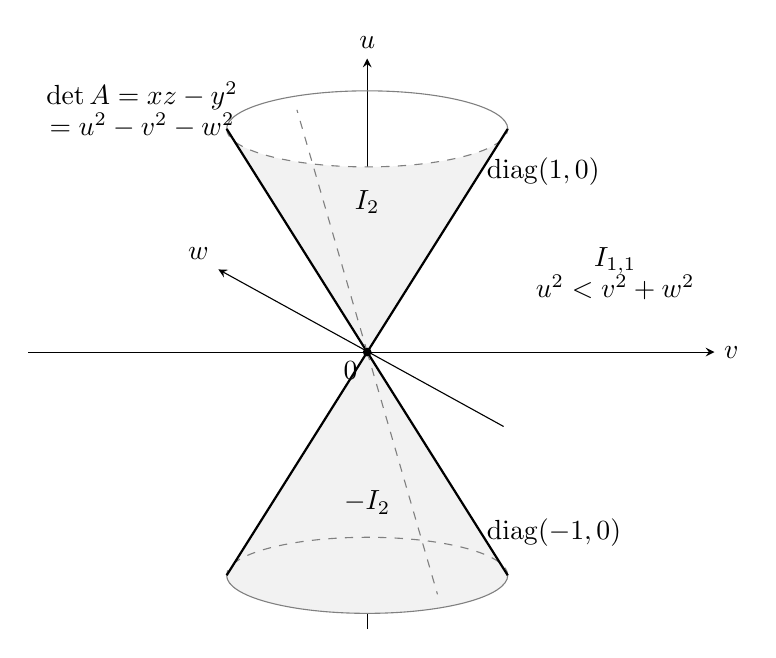
\begin{tikzpicture}[>=stealth,scale=1.05]
  \coordinate (O) at (0,0);
  \coordinate (UT) at (0,2.7);
  \coordinate (LT) at (0,-2.7);

  % Coordinate axes after u=(x+z)/2, v=(x-z)/2, w=y.
  \draw[->,thin] (0,-3.35) -- (0,3.55) node[above] {$u$};
  \draw[->,thin] (-4.1,0) -- (4.2,0) node[right] {$v$};
  \draw[->,thin] (1.65,-0.9) -- (-1.8,1.0) node[above left] {$w$};

  % Light schematic surfaces of u^2=v^2+w^2.
  \fill[gray!10] (O) -- (-1.7,2.7) arc[start angle=180,end angle=360,x radius=1.7,y radius=.46] -- cycle;
  \fill[gray!10] (O) -- (1.7,-2.7) arc[start angle=0,end angle=-180,x radius=1.7,y radius=.46] -- cycle;

  % Back halves of the cross-section ellipses.
  \draw[dashed,gray] (-1.7,2.7) arc[start angle=180,end angle=360,x radius=1.7,y radius=.46];
  \draw[dashed,gray] (1.7,-2.7) arc[start angle=0,end angle=180,x radius=1.7,y radius=.46];
  % Front halves.
  \draw[gray] (1.7,2.7) arc[start angle=0,end angle=180,x radius=1.7,y radius=.46];
  \draw[gray] (-1.7,-2.7) arc[start angle=180,end angle=360,x radius=1.7,y radius=.46];

  % Principal generators of the double cone.
  \draw[thick] (O) -- (-1.7,2.7);
  \draw[thick] (O) -- (1.7,2.7);
  \draw[thick] (O) -- (-1.7,-2.7);
  \draw[thick] (O) -- (1.7,-2.7);
  \draw[dashed,gray] (O) -- (-.85,2.93);
  \draw[dashed,gray] (O) -- (.85,-2.93);

  \fill (O) circle[radius=1.5pt];

  % Six congruence orbits.
  \node at (0,1.82) {$I_2$};
  \node at (0,-1.82) {$-I_2$};
  \node[align=center] at (3.0,.95) {$I_{1,1}$\\[-1pt]$u^2<v^2+w^2$};
  \node[anchor=west] at (1.33,2.18) {$\operatorname{diag}(1,0)$};
  \node[anchor=west] at (1.33,-2.18) {$\operatorname{diag}(-1,0)$};
  \node[below left] at (O) {$0$};

  \node[align=center,anchor=north west] at (-4.0,3.38)
    {$\det A=xz-y^2$\\[-1pt]$=u^2-v^2-w^2$};
\end{tikzpicture}
\end{document}

